\documentclass{report}
\usepackage[a4paper, total={6in, 8in}]{geometry}
\usepackage{amsmath}
\usepackage{bm}
\usepackage{pgfplots}
\usepackage{ amssymb }

%opening
\title{}
\author{Ash}

\begin{document}
	
	\maketitle
	\thispagestyle{empty}
	\newpage
	\thispagestyle{empty}
	\tableofcontents
	\newpage
	\thispagestyle{empty}
	\listoffigures
	\newpage
	
	\chapter{Introduction}
	\textbf{Very brief background}
	Deep learning good for large data set.
	Motivation is to work with less training examples \\
	\textbf{Existing work on meta learning and continuous learning} \\
	\textbf{Gap the literature} \\
	\textbf{Describe the Problem}
	A system that can do continual learning. Refer to this doc:
	https://paper.dropbox.com/doc/Adding-classes-an-existing-classifier-RdKxXHh7M9OWbHvEvCCsV
	We want it to be scalable with respect to the number of classes
	So it should work faster than nearest neighbour based approaches for large number of classes \\
	\textbf{High level how you will solve it and why it is different from existing work} \\
	\textbf{Brief description of experimental setup} \\
	
	
	\chapter{Background}
	\textbf{TODO: Week 2} \\
	\section{Hand Engineered vs Learnt Features}
	\textbf{TODO: Week 2} \\
	Features are a general term for characteristic attributes which exist across all samples in a data-set or domain. These features were traditionally hand-engineered by machine learning experts, carefully selecting the base-components of which the data-set in question appears to comprise. \\
	A fundamental problem with hand-engineered features is that it imposes human knowledge onto a problem to be solved by a computer. Furthermore, key features for complex data such as images and video are incredibly difficult to ascertain -- especially if desiring generic, transferable features. With the rise of neural networks -- specifically CNNs, which will be discussed in detail later -- feature-learning has become the norm. This essentially takes the task of feature engineering and solves it in a data-driven manner.

	\section{Supervised Learning}
	\textbf{TODO: Week 2} \\
	Supervised learning is a machine learning strategy whereby the target solution is presented after each training iteration. This differs from unsupervised learning in that unsupervised learning has no direct target to learn from and is used to find underlying commonalities or patterns in data. \\
	Supervised learning is the most commonly used method for image and video tasks, as typically the objective is to perform tasks where the target is well-defined. Common supervised learning tasks are \textit{image classification} - where the objective is to assign an input image a label from a fixed set of categories; \textit{localisation} - where the objective is to produce the coordinates of an object of interest from the input image; and \textit{detection} - which combines the previous two tasks. \\
	There are a multitude of supervised and unsupervised learning problems, but as with almost all meta-learning strategies I will focus primarily on the supervised task of image classification using neural networks.
	

	\section{Optimisation}
	\textbf{TODO: Week 2} \\
	\subsection{Loss}
	The process of optimising a machine learning system is to present it with a target of some sort -- either in the supervised or unsupervised setting -- and compute a numerical quantity called \textit{loss} or \textit{cost}. The loss is a scalar value which is representative of how "badly" the system has performed inference given the input image. It is the system's objective to minimise this value through some optimisation algorithm. The loss function is specifically chosen for the task at hand, \textit{cross-entropy} being a common choice for image classification tasks and \textit{mean-squared (L2) error}  for localisation. \\
	
	\subsubsection{Symbols}
	Before discussing loss functions, it's important to understand the inputs and outputs of a machine learning system when performing image classification. \\
	For a system that makes predictions between $N$ classes, its input is a vector of image features $\bm{x}$ - usually the raw pixel values. The system's output is a vector $\bm{\hat{y}}$ of length $N$, where each of the output values $\bm{\hat{y}}_i$ is a score for class $i$ being the correct answer. The loss $\mathcal{L}$, as described above, is a function of the predictions $\bm{\hat{y}}$ and the target values $\bm{y}$. \\
	The target values are typically encoded as a \textit{one-hot} vector of length $N$, which is all zeros with a 1 in the position of the correct class. \\
	
	\subsubsection{Softmax}
	As the system's outputs aren't normalised and thus cannot be interpreted as a true confidence measure, the outputs normally go through a softmax function $\sigma$.
	\begin{equation} \label{softmax:1}
	\sigma(\bm{\hat{y}})_i = \frac{e^{\hat{y}_i}}{\sum_{k=1}^{N}e^{\hat{y}_i}} \\
	\end{equation}                                                              
	The softmax function (eq \ref{softmax:1}) squashes the arbitrary scores into a vector such that its values sum to $1$ and are each in the range $[0, 1]$. The resultant values can be interpreted as the probability of the input image falling into each of the classes. \\
	
	\subsubsection{Cross-Entropy Loss}	
	With the machine learning system producing a normalised probability distribution across classes, those values need be compared with the targets to produce a scalar loss value.
	\textbf{TODO TURN INTO WORDS} \\
	Cross-entropy loss, otherwise known as \textit{log loss}, penalises for differences between predicted values and targets, with the penalty growing harsher for further-away predictions as demonstrated in fig \ref{fig:cross-entropy:1}.\\
	For a vector of predictions $\bm{\hat{y}}$ and a one-hot target vector $\bm{y}$, the cross-entropy loss is:
	\begin{equation} \label{cross-entropy:1}
	H(\bm{\hat{y}}, \bm{y}) = - \sum_{k=1}^{N}y_k log(\hat{y}_k) \\
	\end{equation}  
	For the special case of \textit{binary} cross-entropy (as shown in fig \ref{fig:cross-entropy:1}) where number of classes $N$ is 2, the network's outputs are generally reduced to a single scalar value and cross entropy calculated as:
	\begin{equation} \label{cross-entropy:2}
	H(\hat{y}, y) = -(y log(\hat{y}) + (1 - y)log(1-\hat{y})
	\end{equation}
	\begin{figure}[!h]
		\centering
			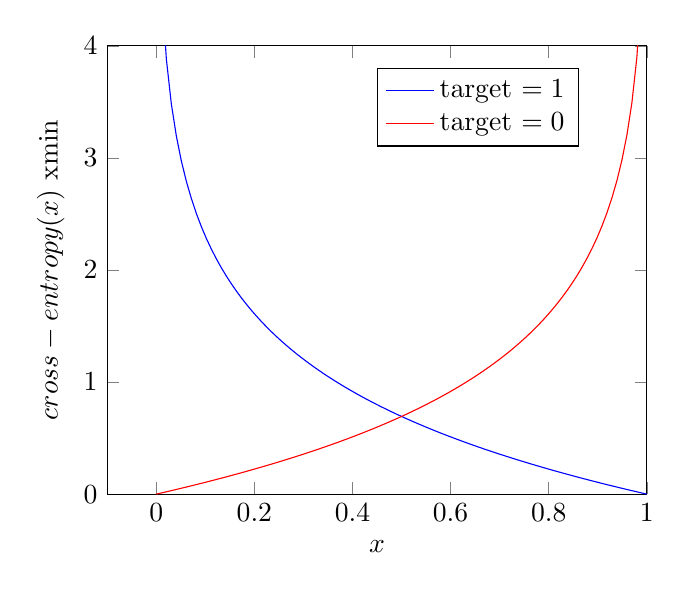
\begin{tikzpicture}
			\begin{axis}[ 
			xlabel=$x$,
			ylabel={$cross-entropy(x)$}
			xmin=0, xmax=1,
			ymin=0, ymax=4,
			legend style={at={(0.5,0.95)},anchor=north west}
			] 
			\addplot[domain=-0.01:1, color=blue, samples=100] 
				{-ln(x)};
			\addplot[domain=0:1, color=red, samples=100]
				{-ln(1 - x)};
			\addlegendentry{target $=1$}
			\addlegendentry{target $=0$}
			\end{axis}
			\end{tikzpicture}
			\caption{Binary Cross-Entropy}
			\label{fig:cross-entropy:1}
	\end{figure}
	
	\subsubsection{Mean-Squared Error (L2)}
	\textbf{TODO: BETTER WORDS} \\
	Mean-squared error is used for regression tasks, where the objective is to predict a quantitative value rather than a measure of probability. L2 loss minimises the average error between between the predictions $\bm{\hat{y}}$ and targets $\bm{y}$, the system learns to make predictions which lie in the mean position of these, which is generally ideal for regression tasks where there is one solution.\\
	\begin{equation} \label{mean-squared-error:1}
	L2(\hat{\bm{y}}, \bm{y}) = \sum_{k=1}^{N}(y_k - \hat{y}_k)^2
	\end{equation}
	
	\subsection{Neural Networks}
	Neural networks are a machine learning architecture that were inspired by the functioning of biological neural networks found in the brain. Studies 
	- Loss curve \\
	- Gradient descent \\
		- Why \\
		- How \\
	
	\subsection{SGD}
	\textbf{TODO: Week 2} \\
	- Why use Sgd
	

	\subsection{Backprop}
	\textbf{TODO: Week 2} \\
	\subsection{Adaptive Optimizers}
	\subsubsection{SGD with Momentum}
	\subsubsection{Nesterov Accelerated Gradient}
	\subsubsection{Adagrad}
	\subsubsection{Adadelta}
	\subsubsection{RMSprop}
	\subsubsection{Adam}
	
	\section{Dealing with Small Training Data Sets}
	\subsection{Overfitting}
	\subsection{Transfer Learning}
	\subsection{Few-Shot Learning}
	\subsection{Meta Learning}
	\textit{Break into meta training, testing, episodes, etc.}
	\section{Continuous Learning}
	\textit{Catastrophic forgetting}
	\section{Modern Deep Learning Architectures}
	\subsection{Convolutional Neural Networks}
	\subsection{Recurrent Neural Networks}
	
	\chapter{Related Works}
	\section{Meta Learning}
	Approaches in meta learning with neural networks are generally groupd into three categories.
	\subsection{Model Based}
	\subsection{Metric Based}
	\subsection{Optimization Based}
	\section{Continuous Learning}
	
	\chapter{Proposal}
	


\end{document}
